\documentclass[oneside,13pt,a4paper]{report}

% Chargement d'extensions
\usepackage[utf8]{inputenc}
\usepackage[french]{babel}
\usepackage{graphicx}
\usepackage[top=3cm, bottom=3cm, left=3cm, right=3cm]{geometry}
\usepackage{amsmath}
\usepackage{amssymb}

% Liens et autres
\usepackage{hyperref}
\hypersetup{
    colorlinks=true,
    linkcolor=black,
	urlcolor=blue,
	pdftitle={Rapport de projet Claims checking},
	bookmarks=true,
}

% Bout de code
\usepackage{listings}
\usepackage{color}

% arabe
\usepackage{arabtex}

\definecolor{mygreen}{rgb}{0,0.6,0}
\definecolor{mygray}{rgb}{0.5,0.5,0.5}
\definecolor{mymauve}{rgb}{0.58,0,0.82}

\lstset{
  backgroundcolor=\color{white},   % choose the background color; you must add \usepackage{color} or \usepackage{xcolor}; should come as last argument
  basicstyle=\footnotesize,        % the size of the fonts that are used for the code
  breakatwhitespace=false,         % sets if automatic breaks should only happen at whitespace
  breaklines=true,                 % sets automatic line breaking
  captionpos=b,                    % sets the caption-position to bottom
  commentstyle=\color{mygreen},    % comment style
  deletekeywords={...},            % if you want to delete keywords from the given language
  escapeinside={\%*}{*)},          % if you want to add LaTeX within your code
  extendedchars=true,              % lets you use non-ASCII characters; for 8-bits encodings only, does not work with UTF-8
  firstnumber=0,                   % start line enumeration with line 1000
  frame=single,	                   % adds a frame around the code
  keepspaces=true,                 % keeps spaces in text, useful for keeping indentation of code (possibly needs columns=flexible)
  keywordstyle=\color{blue},       % keyword style
  language=C++,                    % the language of the code
  morekeywords={*,...},            % if you want to add more keywords to the set
  numbers=left,                    % where to put the line-numbers; possible values are (none, left, right)
  numbersep=5pt,                   % how far the line-numbers are from the code
  numberstyle=\tiny\color{mygray}, % the style that is used for the line-numbers
  rulecolor=\color{black},         % if not set, the frame-color may be changed on line-breaks within not-black text (e.g. comments (green here))
  showspaces=false,                % show spaces everywhere adding particular underscores; it overrides 'showstringspaces'
  showstringspaces=false,          % underline spaces within strings only
  showtabs=false,                  % show tabs within strings adding particular underscores
  stepnumber=1,                    % the step between two line-numbers. If it's 1, each line will be numbered
  stringstyle=\color{mymauve},     % string literal style
  tabsize=2,	                   % sets default tabsize to 2 spaces
}

% Commande pour notation 'NB :' (nota bene)
\newcommand\nb[1][0.3]{N\kern-#1emB : }

% csquotes va utiliser la langue définie dans babel
\usepackage[babel=true]{csquotes}

% pour afficher Schéma au lieu de figure dans les legende des images
\addto\captionsfrench{\def\figurename{Schéma}}

% Informations le titre, le(s) auteur(s), la date
\title{Claims checking}
\author{
    Belkassim BOUZIDI \and
    Chakib ELHOUITI \and
    Massili KEZZOUL \and
    Abdelkader NEDJARI \and
    Ramzi ZEROUAL
}
\date{\today}


\begin{document}
%\maketitle
\begin{titlepage}
	\centering
	{\scshape\LARGE Universite de Montpellier\par}
	{\scshape\Large Rapport de projet\par}
	\vspace{1.5cm}
	{\huge\bfseries Claims checking\par}
	\vspace{2cm}
	{\Large\itshape
		Belkassim BOUZIDI \\
		Chakib ELHOUITI \\
		Massili KEZZOUL \\
		Abdelkader NEDJARI \\
		Ramzi ZEROUAL \\
		\par}

	\vspace{1.5cm}

	{\Large\itshape
		Encadrant :\par
		M\up{r} Konstantin \textsc{Todorov}
		\par}

	\vspace{2cm}

	\begin{figure}[h]
		\begin{minipage}[c]{.46\linewidth}
			\centering
			
\includegraphics[width=1\textwidth]{img/univ-montpellier.png}
		\end{minipage}
		\hfill%
		\begin{minipage}[c]{.46\linewidth}
			\centering
			
\includegraphics[width=1\textwidth]{img/fds.png}
		\end{minipage}
	\end{figure}

	\par\vspace{1cm}

	\vfill

	% Bottom of the page
	{\large \today\par}
\end{titlepage}




% ------------------------------------- %
% Introduction
% ------------------------------------- %

\parskip=5pt
\chapter*{Remerciements}
\vspace{\stretch{1}}
\begin{center}

	Tout d'abord nous souhaitons adresser nos remerciements au corps professoral et administratif de la faculté des sciences de Montpellier qui déploient des efforts pour assurer à leurs étudiants une formation actualisée.

	En second lieu, nous tenons à remercier notre encadrant M\up{r} Konstantin \textsc{Todorov} pour ses précieux conseils et son aide durant toute la période du travail.

	Nos vifs remerciements vont également aux membres du jury pour l’intérêt qu’ils ont porté à notre projet en acceptant d’examiner notre travail.

	Nous remercions M\up{r} Yahia Zeroual pour sa relecture attentive de ce rapport.

\end{center}
\vspace{\stretch{1}}

\parskip=0pt
\tableofcontents

% Espacement entre les paragraphes
\parskip=5pt
% ------------------------------------- %
% Organisation
% ------------------------------------- %

\chapter{Organisation du projet}
\section{Méthodes d’organisation}

Afin de mener à bien le développement du projet, nous avons décidé de travailler un maximum de temps ensemble et de manière très régulière. Nous nous sommes réunis trois à quatre fois par semaine, en vue de faire le point sur l'avancement du projet et de définir les objectifs restants à atteindre.

Ainsi, selon l'état de progression de la conception, nous réalisâmes les tâches en retard durant le week-end pour ne pas cumuler de retard et respecter l'intégralité du cahier de charges.

Toutes les semaines, nous nous sommes réunis avec notre encadrant, M\up{r} Konstantin \textsc{Todorov}. Lors de ces réunions de mises au point relatifs au projet, nous furent prodigués, cela nous a permis de bénéficier de précieux conseils.

\section{Découpage du projet}

Nous avons découpé la réalisation du projet en trois grandes phases :

\subsection{Phase de modélisation}

Durant cette étape, nous nous sommes réunis pour définir les fonctionnalités demandées par le projet. Notamment séparer les fonctionnalités importantes de celles moins importantes. Nous avons également choisi les outils de travail collaboratifs et les principales technologies utilisées, ainsi qu’une première modélisation du projet.

\subsection{Phase de développement}

Durant cette phase, nous avons commencé à implémenter les différentes fonctionnalités que nous avons modélisées lors de l'étape précédente, tout en améliorant la modélisation au fur et à mesure de l'avancement de notre projet. Nous avons notamment réalisé des tests pour les différents modules afin de s'assurer de leur bon fonctionnement.

\subsection{Finalisation du projet}

Cette étape a consisté en la réalisation des tests finaux afin de s'assurer que les différents scripts fonctionnent en toute circonstance et éventuellement corriger les bogues qui peuvent apparaître.

\section{Outils de collaboration}

Afin de s'organiser, nous avons décidé d'utiliser Git à travers le serveur GitLab hébergé par le service informatique de la faculté. En effet le logiciel libre Git a facilité grandement la collaboration entre nous. Le serveur GitLab quant à lui est fourni gratuitement par le service informatique de la faculté.

En ce qui concerne la rédaction de ce rapport, nous avons utilisé \LaTeX, système de composition de documents créé par Leslie Lamport, pour faciliter la rédaction à plusieurs.

\begin{figure}[h]
	\begin{minipage}[c]{.46\linewidth}
		\centering
		
\includegraphics[width=1\textwidth]{img/gitlab.png}
		\caption{Logo du GitLab}
	\end{minipage}
	\hfill%
	\begin{minipage}[c]{.46\linewidth}
		\centering
		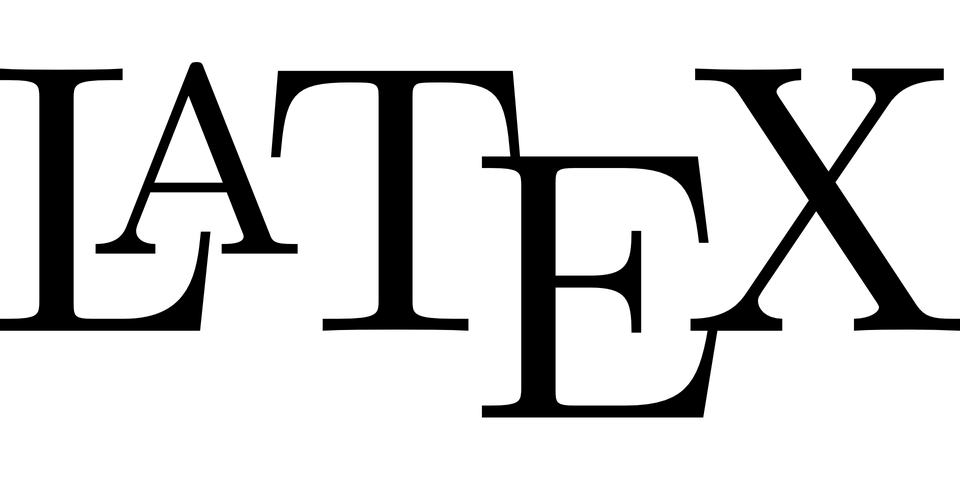
\includegraphics[width=1\textwidth]{img/latex.png}
		\caption{Logo de Latex}
	\end{minipage}
\end{figure}



\chapter{Introduction au sujet}

\section{Fact-checking}

\subsection{Présentation du principe de fact-checking}

Le fact-checking ou le vérification des faits, est une technique consistant à vérifier la véracité des faits et l'exactitude des chiffres présentés dans les médias, les différents réseaux sociaux, les blogs, etc...
Cette notion est apparue aux États-Unis dans les années 1990. Elle a été mise en pratique par des journalistes d'investigation dans le cadre de leur profession, la méthode s'est démocratisée grâce à des logiciels aidant les particuliers à vérifier les faits.

L'entrée officielle du fact-checking en France date de 1995, quand est créée l'association Acrimed, qui se présente comme « l'observatoire des médias ».

En vue de la prolifération très rapide des informations, il devient de plus en plus important de s'assurer de la véracité des informations qui se trouvent partout sur Internet et autres médias. Tant du point de vue de la société que de celui de la recherche. De nombreuses approches récentes dans diverses communautés scientifiques portent sur des problèmes tels que la vérification des faits, la détection de la pertinence ou de point de vue des documents par rapport à des revendications particulières.

\subsection{Présentation de ClaimsKG}

% [1] tsema faut mettre des liens

Le LIRMM \footnote{Le Laboratoire d’Informatique, de Robotique et de Microélectronique de Montpellier} en collaboration avec 2 équipes allemandes (L3S Hannover et l’institut de sciences sociologiques GESIS à Cologne) a construit et mis à disposition la base de connaissance ClaimsKG \footnote{\url{https://github.com/claimskg}} qui regroupe les informations et méta-données provenant d’un grand nombre de sites journalistiques internationaux de fact checking, tels que Politifact\footnote{\url{https://www.politifact.com/}} ou Snopes\footnote{\url{https://www.snopes.com/}}. ClaimsKG est un graphe de connaissances d’assertions annotées et liées qui facilite la création de requêtes structurées sur les assertions, leurs valeurs de vérité (True, Mostly False, etc...), leurs auteurs, date de publication, etc... ClaimsKG est généré par un pipeline entièrement automatisé qui collecte des assertions et des métadonnées à partir des sites de fact-checking, il transforme les données en graphes de connaissances selon un modèle établi, et annote les assertions avec des entités DBpedia (Wikipedia). La base actuelle comprend plus de 32 000 assertions publiées depuis 1996 et est mise à jour régulièrement.

\subsection{Travail à réaliser}

Le sujet du TER consiste en l’enrichissement de cette base de connaissances avec des nouvelles données provenant des sites web suivants :

\begin{description}
	%"فتبينوا" arabe non pris en charge ?????
	\item[Fatabyyano]\footnote{\url{https://fatabyyano.net/}} est un site jordanien en arabe. Fatabyyano (terme en arabe qui veut dire "Alors montrez-le") est la première et la seule plateforme arabe certifiée par l'IFCN \footnote{International Fact-Checking Network : \url{https://www.poynter.org/ifcn/}};
	\item[Vishvas.news]\footnote{\url{https://www.vishvasnews.com/}} est un site Internet de vérification des faits multilingue qui s'engage à combattre la désinformation et les informations erronées.
\end{description}

Le but du TER sera d’identifier les assertions individuelles dans chaque histoire, ainsi que leur label de véracité et par la suite identifier les relations entre elles, ainsi que les relations entre ces histoires. Les données produites par ce projet seront intégrées à la base de connaissance ClaimsKG.

La principale difficulté qu'on s'attend à rencontrer est la gestion des différentes langues proposée par ces sites web. Notamment dans l'identification des différentes relations entre les assertions. En effet afin de reconnaitre les différents mots-clés du sujet traité par les articles, on utilise habituellement TAGME, un puissant outil de reconnaissance d'entités nommées dans un texte. Les langues utilisées par ces sites web ne sont pas prises en charge par cet outil. Il s'agit donc de trouver une alternative afin de reconnaitre ses différentes assertions. Ce problème ainsi que sa résolution seront détaillés plus tard dans ce rapport.

\section{Technologies utilisées}

Nous avons implémenter l'application en Python, choix qui s'impose de lui même car couplé à la bibliothèque BeautifulSoup, il devient très facile de faire du web scraping\footnote{Le web scraping est une technique d'extraction du contenu de sites Web, via un script ou un programme}.

En ce qui concerne la traduction, nous avons choisi d'utiliser Yandex Translator\footnote{\url{https://translate.yandex.com/}}. En effet en vue de la taille des données à traduire, nous n'avons pas pu utiliser l'API de traduction de Google puisque cette dernière devient payante à partir d'un certain nombre de caractères.

Enfin, la reconnaissance des différents entités concernées est faite grâce à l'outil TAGME\footnote{\url{https://tagme.d4science.org/tagme/}} a travers son API python\footnote{Lien Github vers l'api Python de TAGME : \url{https://github.com/marcocor/tagme-python}}.

\vspace{2cm}
\begin{figure}[h]
	\begin{minipage}[c]{.30\linewidth}
		\centering
		
\includegraphics[width=1\textwidth]{img/python.jpg}
		\caption{Logo de Python}
	\end{minipage}
	\hfill%
	\begin{minipage}[c]{.30\linewidth}
		\centering
		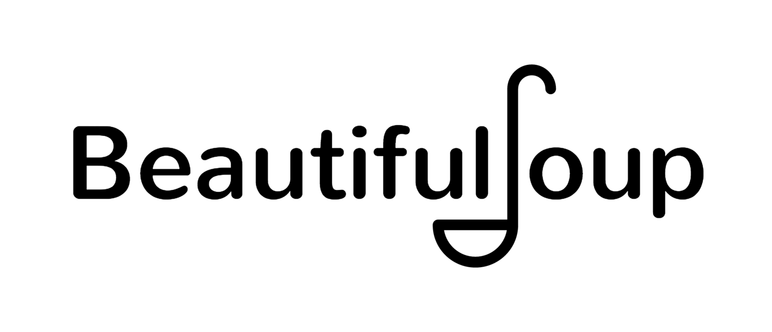
\includegraphics[width=1\textwidth]{img/bs.png}
		\caption{Logo de BeautifulSoup}
	\end{minipage}
	\hfill%
	\begin{minipage}[c]{.30\linewidth}
		\centering
		
\includegraphics[width=1\textwidth]{img/yandex.png}
		\caption{Logo de Yandex}
	\end{minipage}
\end{figure}

\chapter{Conception et implémentation du projet}

\section{Conception et Modélisation}

\subsection{Analyse de ClaimKG}

Lors de cette première phase, le plus important a été de comprendre et s'imprégner du code et de la structure déjà mis en place et mis à notre disposition (Claimskg), comprendre les outils utilisés ainsi que la structure déjà établie.

\subsubsection*{La structure}

Comme le projet est d'une envergure immense, bien comprendre la structure était primordiale afin de respecter un maximum les outils utilisés. Notre encadrant nous à mis a disposition un écrit (que vous trouverez dans le dossier autre/ sous le nom de ClaimsKG.pdf) qui explique la structure globale du projet dont voilà ci-dessous un résumé.

\begin{figure}[h]
	\centering
	\begin{minipage}[c]{.95\linewidth}
		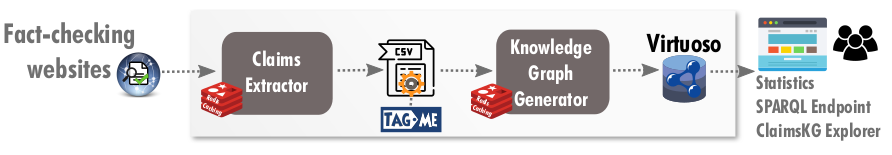
\includegraphics[width=1\textwidth]{img/claim.png}
		\caption{ClaimKG}
	\end{minipage}
\end{figure}

Comme vous pouvez le voir sur le schéma, ClaimsKG est découpé en plusieurs phases. La première consiste à extraire les données brutes à partir de site web de fact-checking et ensuite les structurer afin de produire un fichier CSV. La deuxième phase quant à elle, consiste à faire passer ce fichier CSV dans un générateur de graphes de connaissances\footnote{Knowledge Graph Generator}. Dans notre cas, on s'occupe de la première phase, c'est-à-dire, extraire les données brutes du site web afin de produire le fichier CSV.

Le fichier CSV en question contient l'ensemble des faits traités par un site web. Chaque fait est passé à un script de scraping afin d'extraite chaque information et la structurer. La structure d'un fait est réalisée selon un modèle précis dont voici une partie :

%la faire descendre.
\begin{description}
	\item[rating value] : La valeur de véracité du fait.
	\item[creativeWork author name] : Auteur de la claim.
	\item[creativeWork datePublished] : Date de publication de la claim.
	\item[claimReview author] : Auteur de l'article/analyse de la claim.
	\item[extra entities claimReview] : Les différentes entités présentes dans la review.
\end{description}

Vous trouverez ci-dessous la structuration complète.

\begin{figure}[h]
	\centering
	\begin{minipage}[c]{.95\linewidth}
		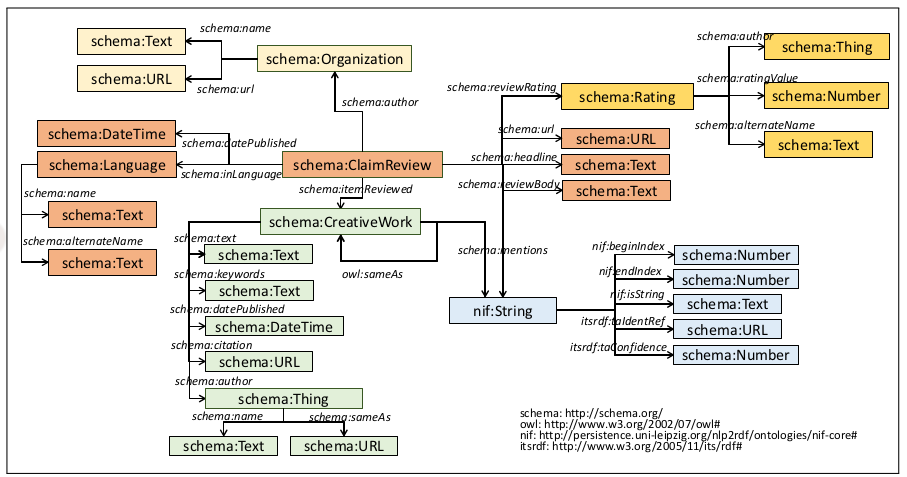
\includegraphics[width=1\textwidth]{img/claimKG.png}
		\caption{Structuration complète d'un fait}
	\end{minipage}
\end{figure}


\subsubsection*{L'implémentation}

Après la partie théorique de l'analyse nous avons commencer à regarder les implémentations déjà faite\footnote{Vous trouverez cette implémentation à cette addresse : \url{https://github.com/claimskg/claimskg-extractor}}. Nous avons analysé les classes principales comme celle de \enquote{Claim.py}, puis comprendre comment l'exécution de l'extraction ce fessait avec \enquote{\_\_init\_\_.py}. nous avons ensuite analysé les différents scripts d'extraction de sites de fact-cheking tel que \enquote{africacheck.py}.

\begin{figure}[h]
	\centering
	\begin{minipage}[c]{.8\linewidth}
		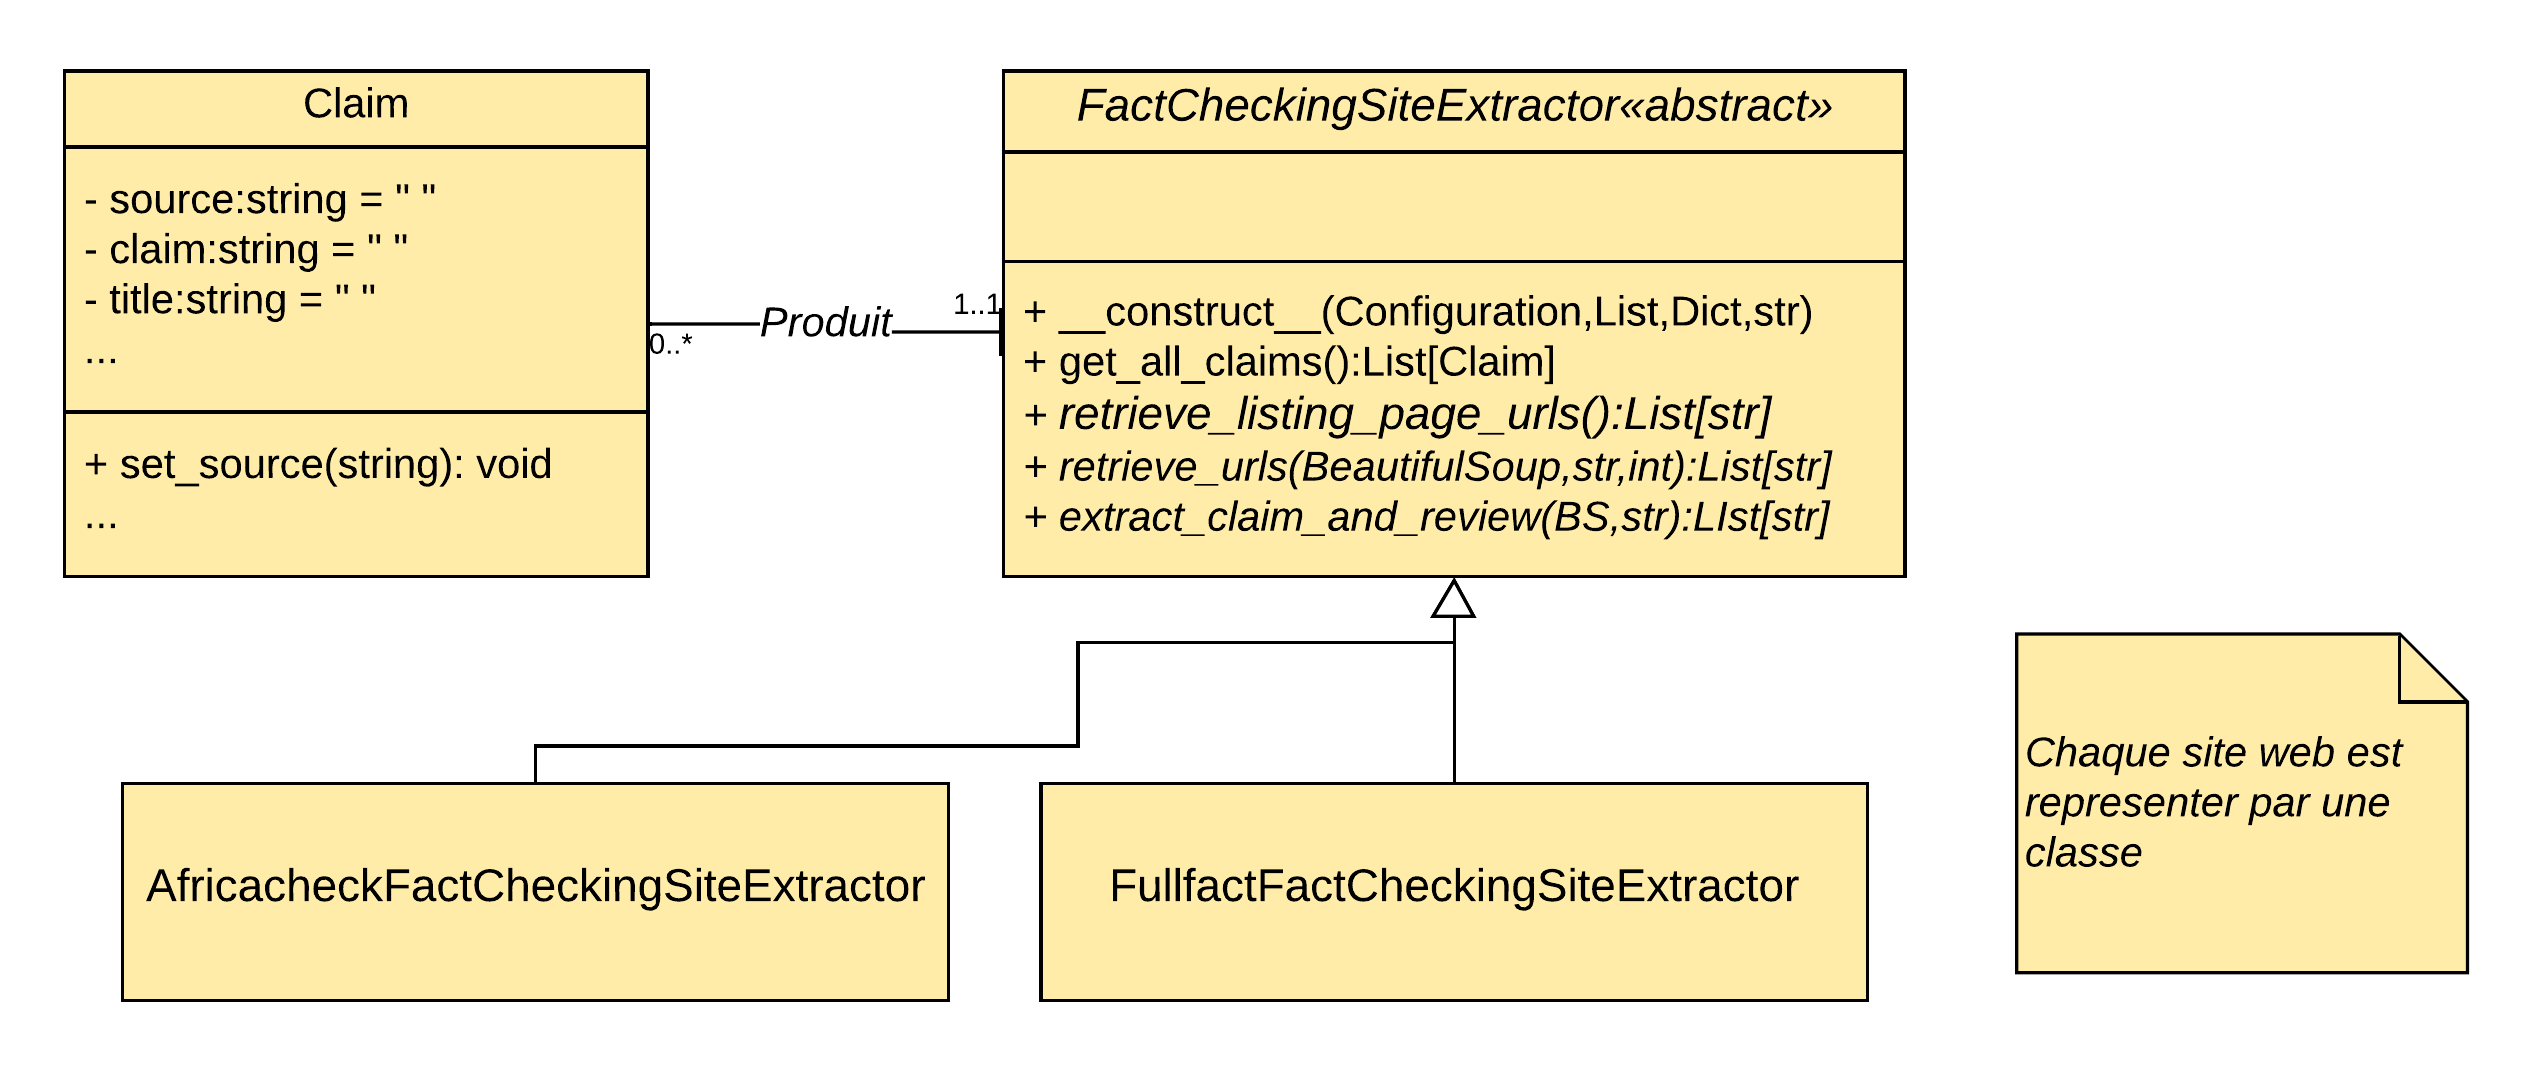
\includegraphics[width=1\textwidth]{img/claimsKG-extractor-uml.png}
		\caption{Structuration de claimsKG-extractor}
	\end{minipage}
\end{figure}


\subsection{Structure des scripts}
% reformuler ces titres
\subsubsection*{Parler des class et un peu d'UML}

% reformuler cette partie
De ce que nous avons compris du projet il fallait écrire une classe qui représente l'extracteur, puis écrire des méthodes d'extraction (extraction du titre, extraction de la claim ... etc. ) sur une page que nous appliquerons sur tout le site via un script python, chaque méthode représente une colonne du fichier csv final où tous les éléments extraits sont stockés, tous les résultats de chaque méthode sont regroupés dans une méthode qui les regroupent dans la classe principale `Claim.py` et c'est sur celle-ci que le script ` init.py ` est appliqué.

parler de l'extraction des liens

puis l'extraction d'une claim

\subsubsection*{Puis parler du format des données que notre prog doit rendre}

L'étape suivante était de trouver un site web respectant les critères de fact cheking ainsi que les critères (une véracité, une claim écrite, un auteur, des tags ... etc) du projet initial (Claimskg), pour apporter un maximum de diversité ainsi que notre contribution personnelle spécifique nous avons décidé avec l'accord de notre encadrant d'extraire les données d'un site d'une langue différente pas encore présente dans le projet, comme tous les étudiants présents dans ce projet ont une connaissance de la langue arabe il a été logique de commencer par cette langue, le seul site officiel de fact cheking en arabe est https://fatabyyano.net/ nous avons donc analysé la structure du site web puis commencé son l'implementation, l'étape d'après fut de trouver comment faire une "named entity recognition" sur les mêmes principes que celle déjà présenté ( TagMe qui renvoi vers des liens wikipedia).

Le second site web sur lequel nous avons travaillé est https://www.vishvasnews.com/, 11 langues différentes sont présentent sur ce site : L'anglais, Hindi, Pendjabi, Ourdou, Bengali, Tamoul, Malayalam, Goudjerati, Télougou, Marathi et L'odia , nous avons analysé la structure du site puis extrait ses données.

\section{Implémentation}

\chapter{Analyse des résultats}

\section{Résultats}
Comme premier résultat du site fatabayyano nous avons obtenu un fichier csv contenant l'url de la claim le rating et sa traduction la claim, la date , le titre, tous les liens présents sur la page et les tags tout cela en langue arabe.
\begin{figure}[h]
	\centering
	\begin{minipage}[c]{.5\linewidth}
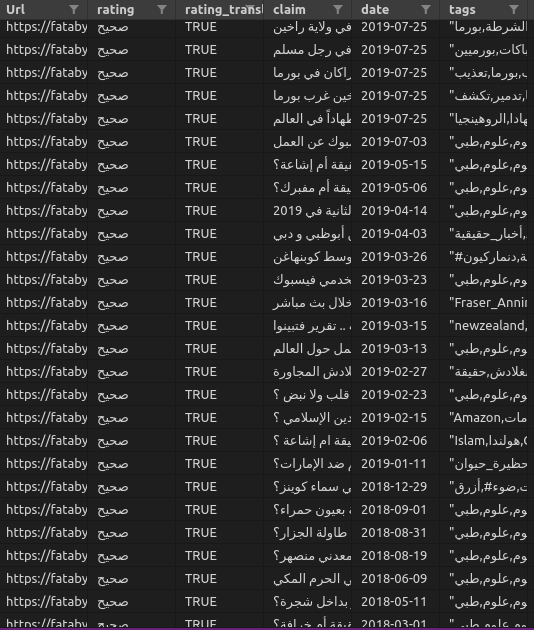
\includegraphics[width=1\textwidth]{img/fatab1.png}
\caption{premier fichier csv obtenu}
	\end{minipage}
\end{figure}

Puis après avoir appliqué le processus de traduction sur la claim et la review et après obtention des entités présentes dedans, deux autres colonnes sont ajoutées contenant les résultats du tagme du projet initial, ces résultats sont les noms attribués par la base de données wikipedia de cettte entité.
\begin{figure}[h]
	\centering
	\begin{minipage}[c]{.5\linewidth}
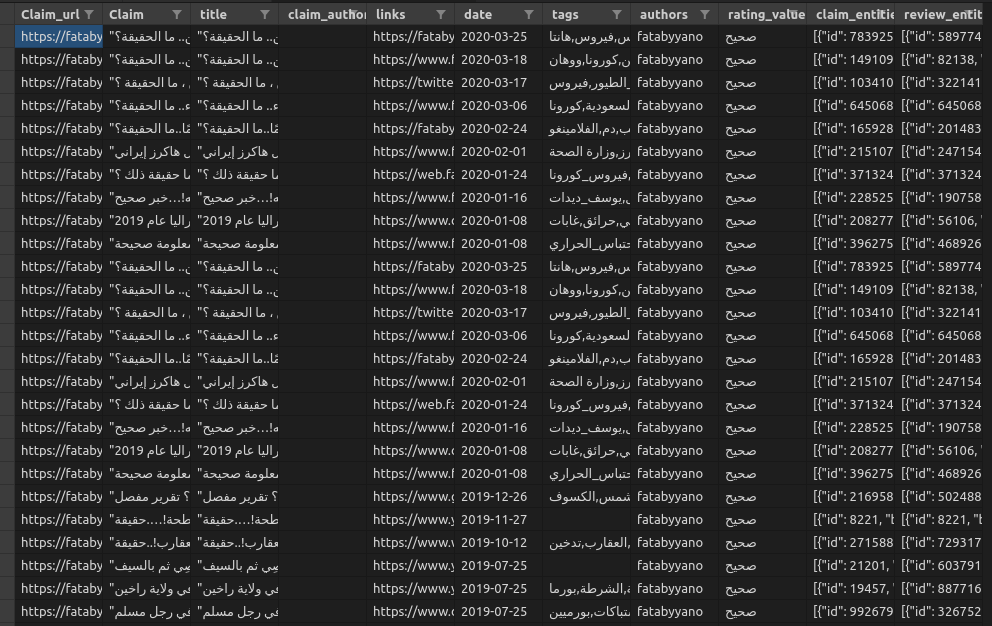
\includegraphics[width=1\textwidth]{img/fatab2.png}
\caption{fichier csv final de fatabayyano}
	\end{minipage}
\end{figure}

Les résultats du second site web "vishvasnews" sont aussi regroupés dans un fichier csv, qui lui est celui généré par le programme du projet initial compte tenu du fait qu'une des langues extraite est l'anglais, les colonnes sont les ratings values, l'auteur de la claim, l'auteur de la review de claim, l'url de la claim, la review, la date, la claim entière, les liens présents, le titre et les tags. Tout cela est rangé par langue l'anglais, Hindi, Pendjabi, Ourdou, Bengali, Tamoul, Malayalam, Goudjerati, Télougou, Marathi puis L'odia puis par catégorie.
\begin{figure}[h]
	\centering
	\begin{minipage}[c]{.5\linewidth}
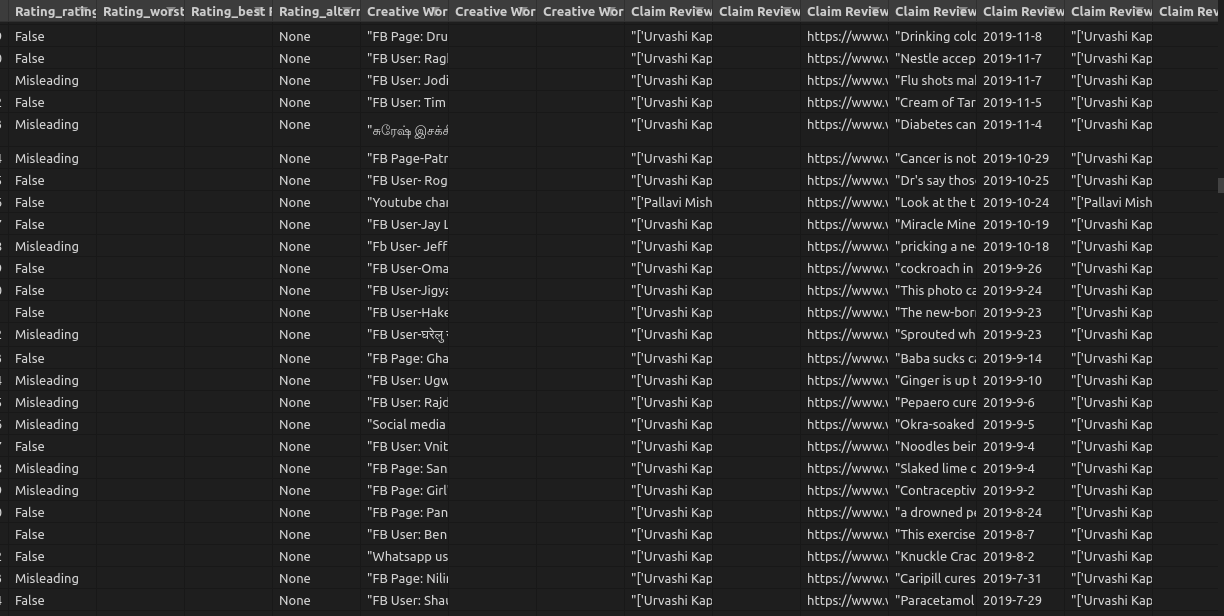
\includegraphics[width=1\textwidth]{img/vishvas.png}
\caption{fichier csv de vishvasnews}
	\end{minipage}
\end{figure}
\section{Problèmes rencotrés}
Le tout premier problème que nous avons rencontré a été lors de l'exécution des scripts d'extraction du projet ClaimsKg. En effet, la majorité des scripts que nous avons essayés ne marchaient plus, certains étaient anciens et n'étaient plus en adéquation avec les mises à jour, soit du projet en lui-même, soit du site web et cause de cela, les bases sur lesquelles nous devions prendre nos marques étaient à prendre avec des pincettes.

Le problème majeur suivant a été de trouver un moyen de faire une « named entity recognition » en langue arabe, car le programme " tagme " ne peut être utilisé sur l'arabe. Nous avons donc cherché des logiciels en open source qui pouvait nous aider à résoudre ce problème, malheureusement, aucun logiciel n'a été satisfaisant; certains nous ont permis comme "Arabic NER" ou " NERAr "de faire des entity recognition, mais sans retourner les liens Wikipedia de ces derniers, d'autres comme " AiDA " qui semblaient être la solution ne fonctionnaient tout simplement pas. Nous avons donc décidé de traduire les claims et leurs reviews afin d'appliquer le programme "tagme", mais là aussi, les API de traduction ne marchaient pas correctement comme googletrans (googletrans est différente de google translate qui n'est pas gratuite) ou étaient limitées par jour comme celle que nous avons utilisé " Yandex ". Le souci avec cette api était que le nombre de caractère traduit quotidiennement était limités.

Le dernier gros problème rencontré quant à lui est le fait que trois des étudiants de notre groupe ont eu des soucis avec leurs machines - deux pc tombés en panne et un chargeur perdu - quelques jours après le début du confinement. Cette contrainte nous a empêché d'aller aussi loin dans la réalisation du projet et nous a retardé sur l'avancement global.
\chapter{Bilan et conclusions}

\section{Ce qu'on a fait et pas fait}

\section{Perspective}


% ------------------------------------- %
% Annexes
% ------------------------------------- %

\appendix
\chapter{Annexe}



\end{document}
